\documentclass{scrartcl}
\usepackage{geometry}
\usepackage{csquotes}
\usepackage{hyperref}
\usepackage{graphicx}
\usepackage{float}
\usepackage{subcaption}
\usepackage{amsmath}
\graphicspath{ {images/} }

\geometry{legalpaper, portrait, margin=1in}
 
\title{Harvard University, John A. Paulson School of Engineering and Applied Sciences \newline}
\subtitle{CS236r Final Project\\ Computational Results For Peer-Prediction and Crowdsourced Judgement Elicitation}
\author{Virgile Audi (vaudi@g.harvard.edu)\\
		Charles Liu (cliu02@g.harvard.edu)}

\begin{document}
 
\maketitle
\section*{Introduction}

A common theme throughout the course is to question the practicality of mechanisms discussed in class. For our presentation of \emph{Crowdsourced Judgement Elicitation with Endogenous Proficiency} and \emph{Eliciting Informative Feedback: The Peer-Prediction Method}, we found the mechanisms relied on strong assumptions that were generally unrealistic. Also, as seen in the second homework with specifying learning rates, in many situations a model can be very sensitive to its parameterization. Difficulties in finding proper parameters can also be viewed as a potential flaw of the mechanism, making it unsuitable for use in a practical setting. For our final project we wanted to take a deeper look at the two mechanisms, relax their assumptions, and see if the mechanism can be modified to achieve similar results. All work can be found at \url{https://github.com/chuckyouliu/Crowdsourced-Elicitation}.

\section{Crowdsourced Elicitation}

The \emph{Crowdsourced Judgement Elicitation with Endogenous Proficiency} paper dealt with a model that incorporated three variables: effort, proficiency, and truthfulness. A user would be given a set of tasks, with each task having a binary type H or T. A user first has the binary option of giving full or no effort. On no effort, the user reports H/T based on a random coin flip. On full effort, the user then has a probability corresponding to his proficiency of correctly interpreting the event. Finally, he can report his signal either truthfully or untruthfully. 

An example use case for this kind of mechanism would be in grading assignments for massive open online courses (MOOCs). If there was a need for graders, e.g. assignments with non-numerical or multiple choice answers, it would be infeasible for a staff to consistently grade answers from thousands of students. Instead, having peer grading would be a natural solution conditional on the fact that students will take the time to grade the assignments and truthfully report the scores.

\subsection{Computational Results of Paper}

We first confirmed the results from the paper computationally, given all of their assumptions. The main benefit to this mechanism was that the maximum reward was achieved in the equilibrium where everyone gave full effort and reported truthfully, whereas giving no effort resulted in an expected reward of 0. Giving full effort and reporting untruthfully is also an equilibrium, however this can be remedied by having some ``known'' truthful users put into the mechanism. One of the stronger results from the paper was Lemma 8:
 
\begin{displayquote}
Suppose the probability of agent i using strategy (1, X) is $\delta$ and strategy $(0, r_i)$ is $1-\delta$ for each task $j \in J(i)$. Suppose i'’s potential reference raters $r_j (i)$ use strategies (1, X) and $(0, r_{r_j} (i))$ with probabilities $\epsilon_{r_j}(i)$ and $1-\epsilon_{r_j}(i)$ respectively, for each task $j \in J(i)$. If $\epsilon_{r_j}(i) > 0$ for any reference rater with proficiency $p_{r_j} (i) > \frac{1}{2}$, then agent i has a (strict) profitable deviation to $\delta'=1$, i.e., to always using strategy (1, X), for all values of $r_i \in [0,1]$
\end{displayquote}

\begin{figure}[H]
	\caption{Computational results of different equilibriums vs. other strategies}
	\centering
	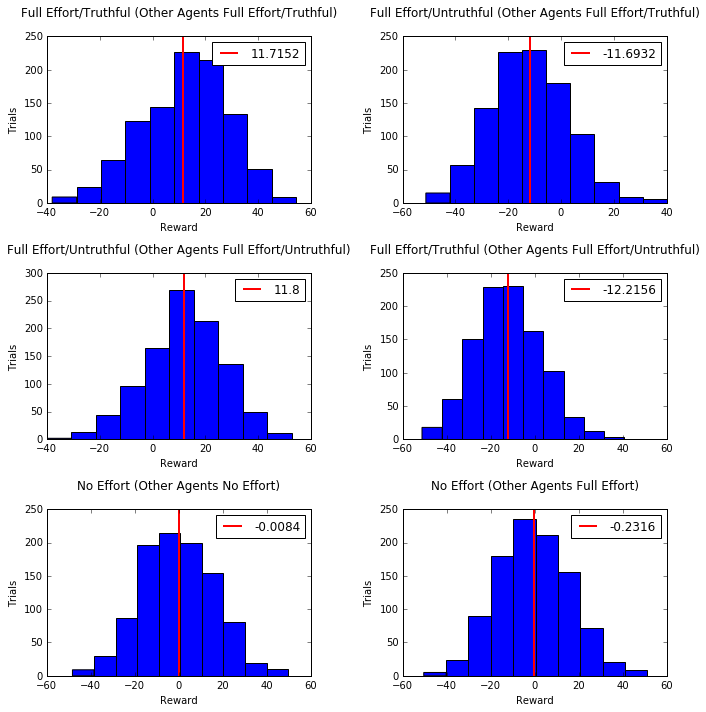
\includegraphics[width=1.0\textwidth]{cs_equilibriums}
\end{figure}
\begin{figure}[H]
	\caption{Computational results of Lemma 8}
	\centering
	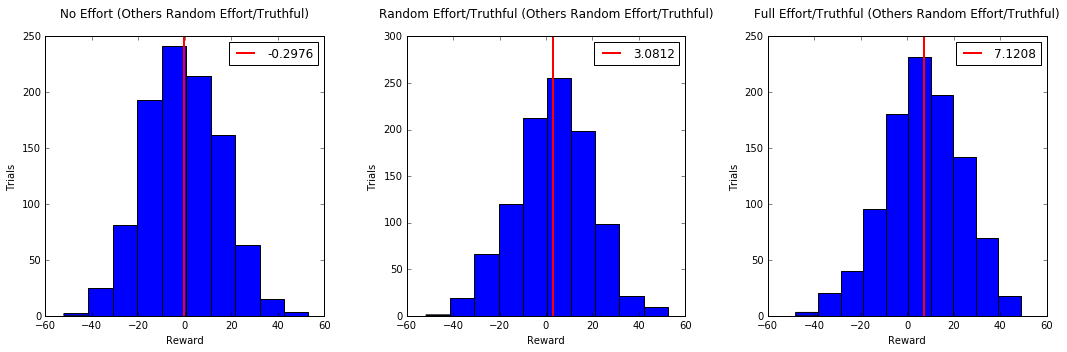
\includegraphics[width=1.0\textwidth]{cs_lemma8}
\end{figure}

Figure 1 is a summary of the main results and Figure 2 of Lemma 8. In each scenario, there were 100 tasks and 20 agents each performing 10 tasks. Simulations were run 1000 times, rewards were scaled by 10, and no costs were factored into the model. All agent proficiencies were randomly assigned between 0.5 and 1.

\subsection{Continuous Effort}

The paper also noted that all results could be extended to the case of a continuous effort distribution where proficiency increased linearly. For a given agent with max proficiency $p_m$, proficiency for a given effort level $e$ was calculated as:

\begin{eqnarray*}
	prof(e) = 0.5 + e*(p_m - 0.5)
\end{eqnarray*}

This maintains the properties of the binary effort case: when effort is fully given your proficiency corresponds to the max proficiency, and when no effort is given your proficiency is in effect a random coin flip. To test that giving full effort was still an equilibrium, we randomly assigned effort levels to each agent. Then iteratively, we would select one agent and perturb its effort level up and down by 0.05 and move the agent's effort level to whatever returned the highest reward. No costs were factored in and rewards were scaled by a factor of 10, similar to the original results.

\begin{figure}[H]
	\caption{Computational results from having continuous effort}
	\centering
	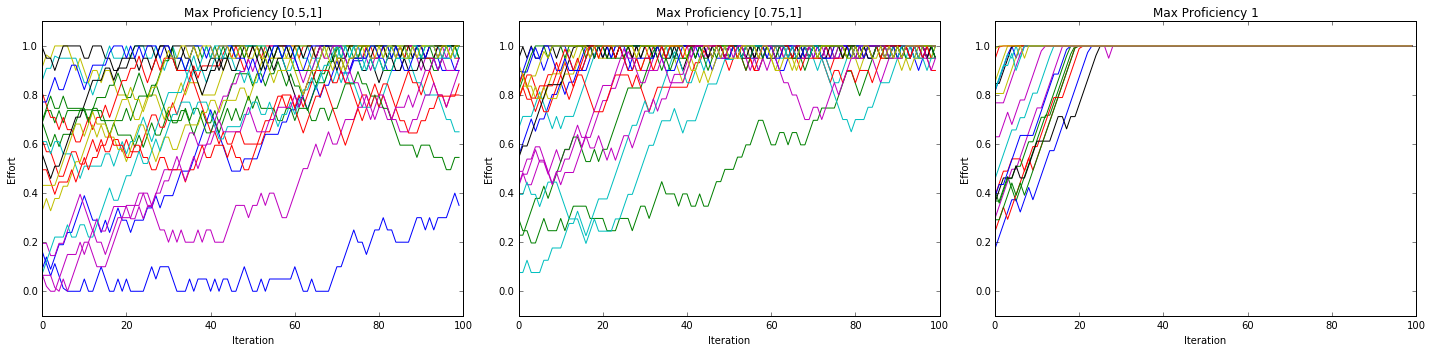
\includegraphics[width=1.0\textwidth]{continuous_effort}
\end{figure}

An equilibrium at full effort is generally reached, but the convergence is not immediate for agents with a lower max proficiency. Figure 3 displays the trace of efforts for each agent under three scenarios:
\begin{itemize}
	\item Max proficiencies between 0.5 and 1
	\item Max proficiencies between 0.75 and 1
	\item Max proficiency of 1
\end{itemize}
Convergence is immediate in the case where max proficiency for each agent is 1, but the more relaxed case sees a more varied strategy with a few agents not approaching giving full effort. For those agents in the last 30 iterations who gave less than .8 effort, the average maximum proficiency of the agent was .616.

\subsection{Cost Reporting}

Although not ideal, it may be possible to enforce some minimum proficiency level of an agent beyond .5 so as to ensure a faster convergence to full effort as an optimal strategy. However, even with a scaling factor of 10 the average reward for an agent in the full effort/truthful equilibrum was only around 12. This mechanism already isn't entirely rational as it is possible for an agent to experience negative rewards, incurring any kind of cost would require a much larger scaling factor for the reward. The paper points out that all results from the paper hold when costs scale linearly to effort, but it would be more interesting to test under different, perhaps convex, cost curves. 

However, computationally it becomes the case that either the costs outweight the benefit of reporting truthfully and the optimal strategy is to give no effort or the reward scaling factor is so large that the costs are negligible resulting in the same results as the paper regardless of the cost curve. As seen from the results in Figure 1, the rewards have quite a lot of variance, so having a large scaling factor to account for costs could potentially lead to very high (and low) rewards. Altogether, it would be nicer to have a modified mechanism that accounted for costs irrespective of the paper's main reward function.

\subsubsection{Take It Or Leave It Crowdsourced Elicitation}
The Take It Or Leave It mechanism that was introduced in class involved asking for a cost from a user, sampling from a distribution, and conducting the survey from the user only if the sample was higher than the user's cost. The mechanism was both truthful and individually rational. It is useful in our case in that we'd like to ask an agent for a cost to reimburse for reporting a task, but we would obviously want a truthful reporting of the cost. Using TIOLI, we introduce a modified crowdsourcing mechanism:

\begin{enumerate}
	\item Distribute tasks to all agents in usual way
	\item For each task, obtain a sample $p$
	\item For each agent, ask for a reported cost
	\item Remove tasks for agents where reported cost is higher than corresponding $p$
	\item Remove tasks for agents who don't have a reference rater or sufficient non-overlapping tasks
	\item Conduct crowdsourced mechanism and then add additional sample $p$ as reward for each task
\end{enumerate}

Finally, if we were to estimate the true signal for a task (e.g. true grade for a student from his peers' grades), we can first estimate the effort given by the agents via their reported cost. If there were some information about each agents' maximum proficiency, we could calculate the probabilities of their reports given the true signal of the task and see which signal is higher.

This mechanism would still incentivize telling the truth as reimbursing the cost gives no incentive to be untruthful and the reward function would still incentivize being truthful if there are other truthful agents. However, one's expected return for giving no effort is no longer 0 as an agent will receive a reimbursement for completing every task.

 \begin{figure}[H]
	\caption{Take It Or Leave It Crowdsourced Mechanism}
	\centering
	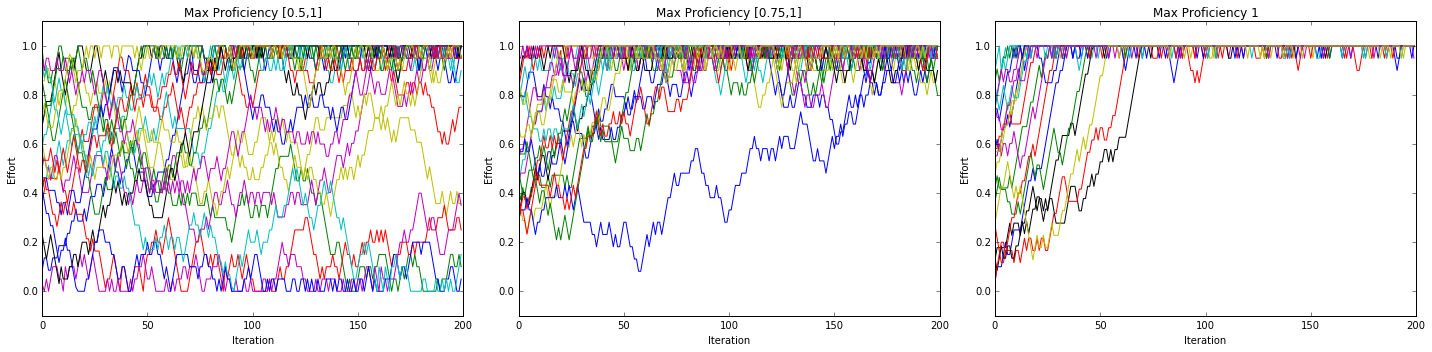
\includegraphics[width=1.0\textwidth]{tioli_effort}
\end{figure}

As Figure 4 shows, the agents are still generally progressing towards telling the truth when proficiencies are high, but in the case of only between 0.5 and 1 the strategies fluctuate heavily. Costs were set equal to effort level, and samples were drawn from a normal distribution with mean 2 and standard deviation 0.5. All other settings were the same as those from Figure 3.

If agent's utility functions aren't linear, they may be fine with gaining some utility for providing no effort. It is also possible that a task has no agents reporting it, though in very large settings this is unlikely. The choice of the distribution becomes very sensitive, but in general the results looked similar with various price distributions (even fixed price) above the maximum cost. We think this is preferable to simply scaling the reward factor of the original mechanism as there are more reasonable bounds on the possible reward given out to reimburse costs whereas as seen in the original computational results, rewards can be quite varied.

\subsubsection{Differing Cost Curves}
Whereas previously the choice of the scaling factor for rewards resulted in either dominating the costs or being dominated and subsequently the optimal strategy went to full or no effort, now with the take it or leave it mechanism varying proficiency curves can be more closely examined.

 \begin{figure}[H]
	\caption{Cost Curve Effects}
	\centering
	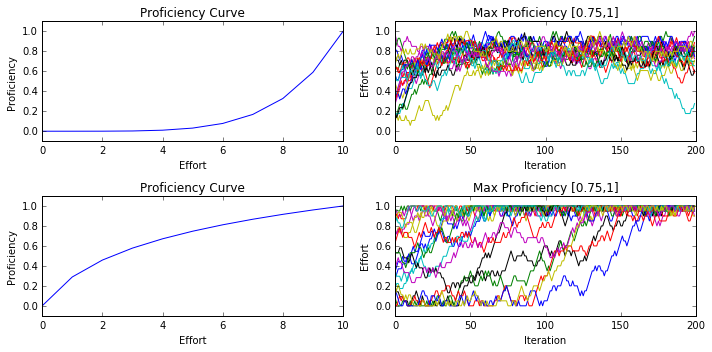
\includegraphics[width=1.0\textwidth]{cost_curves}
\end{figure}

Figure 5 shows a new proficiency curve corresponding to the effort given (and consequently the cost which are linear to effort). We see that there is no longer a convergence to fully telling the truth in the convex case, whereas the convergence seems to happen in the concave case albeit slowly.

\section{Peer Prediction}

We now focus on a second mechanism to elicit truthful reports from agents, i.e. peer prediction. 

\subsection{The Setting}

We consider a group of $n\geq2$ rational, risk-neutral and self-interested agents. The objective of the mechanism is to ellicit for each of these agents $i$ a signal $s_i \in \{1,..., k\}$, which corresponds to an agent's perception of a true state $T \in \{1, ..., m\}$. To translate this set-up in a more practical example, we can imagine multiple agents buying a camera from Amazon. This camera can either be one of two true state: "good" or "bad" quality. The goal is to elicit the perception of the buyers which can be either: "satisfied", "indifferent" or ''disappointed". In order to elicit these signals, we as mechanism designers, need to incentivise the agents by creating a reward function.\\

In order to build this reward function, we need to adopt a probabilistic approach, and suppose that each agent has some prior knowledge of how true states are distributed, represented by $P_i(T=t)$, and how he percieves his signals given a state, denoted by $P_i(S = s | T = t)$. The assumptions one makes on how these signals are distributed, and what information is common or private knowledge will influence the choice of mechanism and will be the focus of the following parts.

\subsection{The Classical Approach}

The classical approach to peer prediction was introduced by Miller et al. (2005). In their paper, the authors make the following assumptions:

\begin{itemize}
\item Raters have common prior over types i.e. $P_i(T = t) = P(T = t) \quad\forall i$,
\item Conditional on the product’s type, raters’ signals are independent and identically distributed,
\item Both the mechanism administrator and the raters have common knowledge of the probability of reporting a signal given a type of a product.
\end{itemize}

Given these strong assumptions, the mechanism is designed as follows:
\begin{enumerate}
\item The center asks each rater to announce his/her signal $s^i$
\item The center assigns a reference rater $j$ to each agent $i$ with $i\neq j$,
\item The center rewards agent $i$ by using a scoring rule such as the logarithmic scoring rule:
$$R(s^j|s^i) = \log p(s^j|s^i)$$
\end{enumerate}

Propositon 1 in Miller et al. proves that truthful reporting is a strict Nash equilibrium. Nevertheless, as one can observe in step 3, it is crucial in order to reward each agent given their reports, that the mechanism knows the priors and distributions of signals given types ! 

\begin{figure}[H]
\caption{Computational verification of Property 1}
\begin{subfigure}{0.4\textwidth}
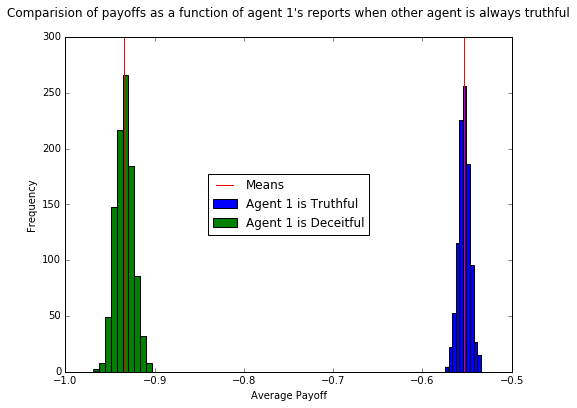
\includegraphics[scale=0.4]{pp_1}
\end{subfigure}
\hspace{0.1\textwidth}
\begin{subfigure}{0.4\textwidth}
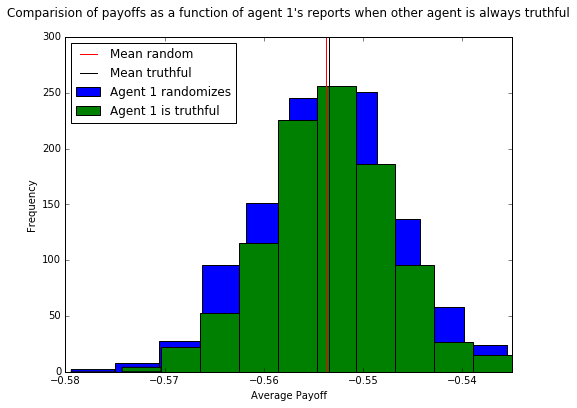
\includegraphics[scale=0.4]{rand}
\end{subfigure}
\end{figure}
These assumptions appeared to us as the most unrealistic. Our intent is to relax these assumptions and see if we can still use the same mechanism. Let's first relax the assumption that agents have identical signal distributions given tasks. We nevertheless maintain the assumptions that everything is common knowledge to both participants and the mechanism since otherwise the latter would not be able to reward agents. We simulated 1000 experiments where two agents are asked to report one of two potential signals given two true states. These agents had different signal distributions. 

\begin{figure}[H]
\caption{Relaxing Assumption 2}
\begin{subfigure}{0.4\textwidth}
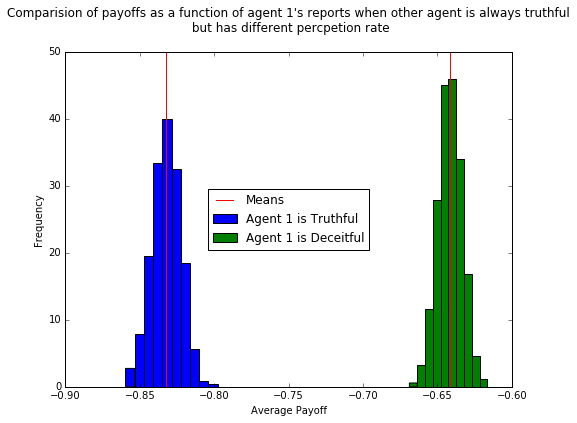
\includegraphics[scale=0.4]{pp_2}
\end{subfigure}
\hspace{0.1\textwidth}
\begin{subfigure}{0.4\textwidth}
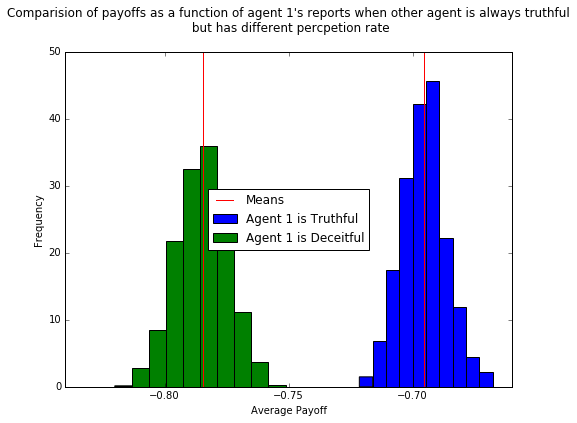
\includegraphics[scale=0.4]{pp_3}
\end{subfigure}
\end{figure}

On the left hand side of figure 8, agent 1 had rather similar signal distributions (only perturbed by a little noise) to agent 2. On the right hand side, agent 1 was much less proficient at perceiving a higher signal given a type that agent 2. In both cases, agents knew about their proficiency and how it compared to the other agent's. These experiments shows that reporting the opposite of the signal perceived can in fact yield higher rewards on average than truthful reporting. A more realistic approach to peer prediction seems to break the mechanism presented by Miller et al. We now present a mechanism that allows a relaxation of the common knowlodge and common priors by introducing the notion of privacy.

\subsection{Private-Prior Peer Prediction}

This mechanism was introduced by Witkowksi et al. in 2012. This mechanism deviates from the previous one in two ways:
\begin{itemize}
\item Agents have their own beliefs about the true states (even the number can differ) and how signals given states are distributed,
\item This information is private to each agent, i.e. neither the mechanism nor the other agents have access to this information.
\end{itemize}

The assumptions made by Witkowsky seem therefore much more realistic than Miller's omniscient mechanism. However, the results presented in the 2012 paper were limited to the case where agents were asked to report one of two signals ("good" or "bad", "Like" or "Dislike", etc.), denoted by $\{0,1\} = \{l,h\}$. The mechanism is implemented as follows:

\begin{enumerate}
\item Assign to agent $i$ a reference agent $j$
\item Ask agent $i$ for his/her prior signal belief $y_i = P_i(h)\,\in\,[0,1]$ that another agent will receive a high signal
\item After observing his/her signal, ask agent $i$ the posterior signal belief report $y_i' \neq y_i$ that another agent will receive a high signal
\item Infer agents implicit signal $x_i$ by:
\[x_i = \begin{cases}
    h,& \text{if } y_i'\geq y_i\\
    l,              & \text{otherwise}
\end{cases}
\]
\item Reward agent $i$ by:
$$u_i = R(y_i,x_j) + R(y_i',x_j)$$
\end{enumerate}
where $R$ is a strictly proper scoring rule and $x_j$ is agent $j$'s implicit signal. To ensure individual rationality, it is suggested to use the normalised binary quadratic scoring rule $R_q$:
\begin{align*}
R_q(y,1) &= 2y-y^2\\
R_q(y,0) &= 1-y^2
\end{align*}

Under the assumption of temporal separation (possibility of asking an agent for his reports at two distinct moment in time), and admissibility of beliefs, then this mechanism is strictly \emph{ex post subjective incentive compatible}, i.e. reporting truthful prior and posteriors is an equilibrium.\\

We wished to investigate numerically this claim. We simulated multiple "experiments" with two participants with different priors over signals and signals. This mechanism gives the possibility to each agent to report untruthfully at two different stages, i.e. his prior and posterior. We tested 3 scenarios where agent 1 lies about his first, second or both reports.

\begin{figure}[H]
\caption{Private-Prior PP}
\begin{subfigure}{0.4\textwidth}
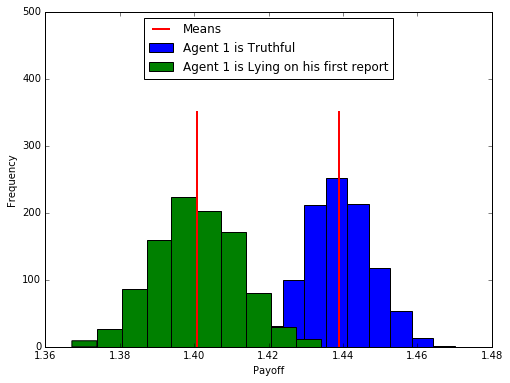
\includegraphics[scale=0.4]{images/pp_first}
\end{subfigure}
\hspace{0.1\textwidth}
\begin{subfigure}{0.4\textwidth}
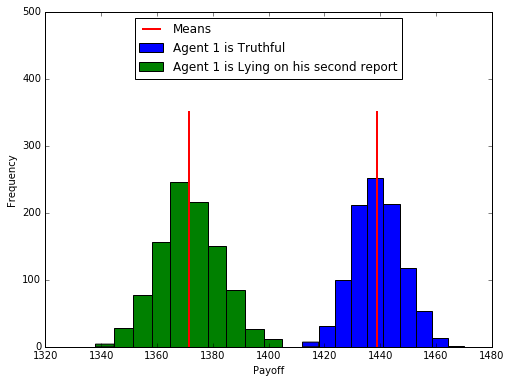
\includegraphics[scale=0.4]{images/pp_second}
\end{subfigure}
\end{figure}
\begin{figure}[H]
\centering
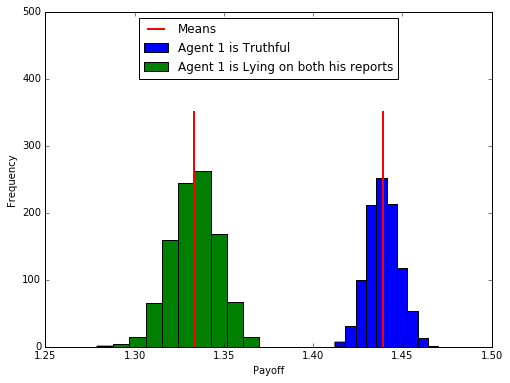
\includegraphics[scale=0.5]{images/pp_both}
\end{figure}

Emperical experiments confirmed the results presented in the paper. However, Miller's paper did not constrained the use of their mechanism to the 2-signal case, we therefore tried to adapt Witkowski mechanism to a 3-signal situation.

\subsection{The 3-signal case}

If Witkowksi limits his analysis to only two signals, it is because he relies on this crucial point to infer the implicit signal for each agent. Indeed, observing a high signal would have for consequence to increase the posterior belief  of another agent receiving a high signal. When dealing with more than two signals, this relation is not true anymore. For instance. Consider an agent that has prior over 2 states:
$$P(T = 1) = 0.3 \text{ and } P(T=2) = 0.7$$
and condition distribution of signals:
$$P(s = 1 | T = 1) = 0.7,\, P(s = 2 | T = 1) = 0.1, \, \text{and } P(s = 3 | T = 1) = 0.2$$
$$P(s = 1 | T = 2) = 0.1,\, P(s = 2 | T = 2) = 0.2, \, \text{and } P(s = 3 | T = 2) = 0.7$$
This yields prior over signals equal to:
$$P(s = 1) = 0.28, \, P(s=2) = 0.17,\text{ and } P(s=3)=0.55$$
If agent observes a signal of 2, then his posterior distributions is therefore:
$$P(s = 1) = 0.169, \, P(s=2) = 0.183,\text{ and } P(s=3)=0.649$$
and if he observes 3, then:
$$P(s = 1) = 0.177, \, P(s=2) = 0.176,\text{ and } P(s=3)=0.646$$
It is therefore unclear how to conclude which is his signal when comparing these posteriors with the priors.\\ 

We therefore propose the following mechanism:
\begin{enumerate}
\item Assign to agent $i$ a reference agent $j$
\item Ask agent $i$ for his prior belief distribution $y_i$
\item After observing the signal, ask agent $i$ for his posterior belief distribution $y_i'$ as well as his signal $x_i$
\item Reward agent $i$ by:
$$u_i = R(y_i,x_j) + R(y_i',x_j)$$
\end{enumerate}
where $R$ is the classical quadratic scoring rule $R(\mathbf{y},i) = y_i -  \mathbf{y}\cdot\mathbf{y}$.\\

In this set-up, the agent would not have a reason to report a wrong signal as his reward is not based on this report but on his beliefs. If we had trouble proving formally that this mechanism would ellicit the truth theoretically, an informal argument for it would be to use that R is a strictly proper scoring rule.\\

\begin{figure}[H]
\caption{Private-Prior with 3 signals}
\begin{subfigure}{0.4\textwidth}
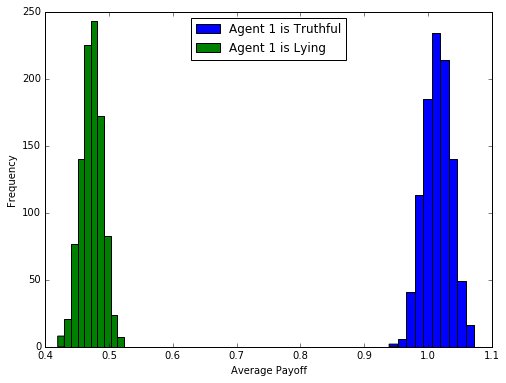
\includegraphics[scale=0.4]{images/3_1}
\end{subfigure}
\hspace{0.1\textwidth}
\begin{subfigure}{0.4\textwidth}
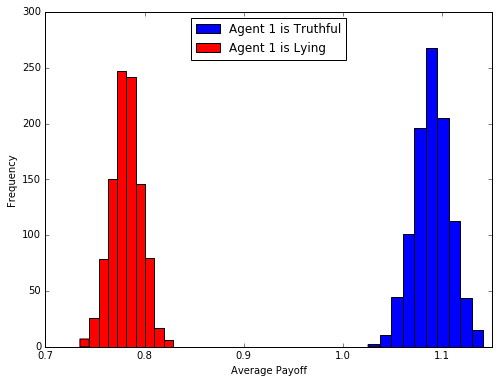
\includegraphics[scale=0.4]{images/3_2}
\end{subfigure}
\end{figure}
\begin{figure}[H]
\centering
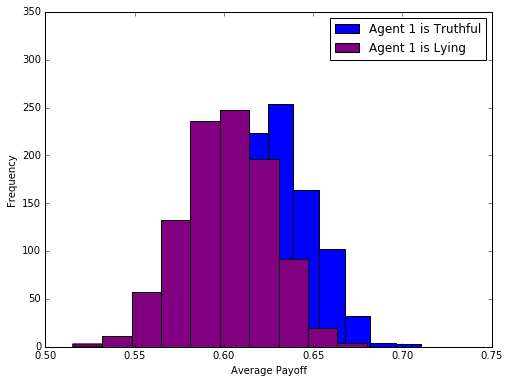
\includegraphics[scale=0.5]{images/3_3}
\end{figure}

The postulate of truthful ellication seems to hold under different similutations, where agents have different priors, and have different lying strategies. Nevertheless, this mechanism could be difficult to implement as it can appear to be quite cumbersome for the agents to report distributions.\\

\section{Conclusion}
In this project, we have presented methods to relax assumptions that made the mechanisms of crowd-sourcing and peer-prediction presented in class difficult to apply in real life. Relaxing assumptions is no easy task and these mechanisms seems far from being fit to reality. The limitation to the 2-signal case is an example of this and we would have benefited from more time to carry out more rigorous extensions of such mechanisms.

\section*{References}
\begin{enumerate}
	\item \emph{Crowdsourced Judgement Elicitation with Endogenous Proficiency}, A. Dasgupta \& A. Ghosh (\url{http://www.arpitaghosh.com/papers/elicit_arxiv_2.pdf} \label{itm:1})
	\item \emph{Eliciting Informative Feedback: The Peer-Prediction Method}, N. Miller, P. Resnick, \& R. Zeckhauser, 2005 (\url{http://www.hks.harvard.edu/fs/rzeckhau/elicit.pdf} \label{itm:2})
	\item \emph{Peer Prediction without a Common Prior}, J. Witkowski, D. Parkes, 2012 $\quad$
	(\url{http://www.eecs.harvard.edu/econcs/pubs/witkowski_ec12.pdf} \label{itm:3})
	\item \emph{Conducting truthful surveys, cheaply}, A. Roth, G. Schoenebeck, Proceedings of the 13th ACM conference on Electrical Commerce, 2012, \quad (\url{http://arxiv.org/pdf/1203.0353v1.pdf})
\end{enumerate}
\end{document}